% Propósito: enseñar a comparar morfologías de timpanogramas sin convertirlas
% en diagnósticos ni presentar límites normativos.
% Origen: definición de timpanograma de la sección
% \ref{sec:u8-timpanometria}. Curvas sintéticas normalizadas:
% Y_N(x)=0.15+0.85 exp[-((x-x_0)/0.65)^2] para los picos,
% con x_0=0 y x_0=-1.15; el trazado plano usa Y_N=0.25.
% La coordenada x es sólo una posición esquemática de presión y no se convierte
% en valores de daPa. No hay datos medidos, normas ni intervalos de referencia.
% Descripción accesible: tres paneles comparten un eje vertical de admitancia
% normalizada y un eje horizontal de presión en decapascales. El primero tiene
% un pico centrado, el segundo es plano y el tercero tiene un pico desplazado
% hacia presiones negativas. Una nota indica que la forma no identifica por sí
% sola una patología.
% Validación prevista: comprobar las funciones, la normalización, el sentido de
% la presión, las unidades y que ningún panel incluya valores normativos.
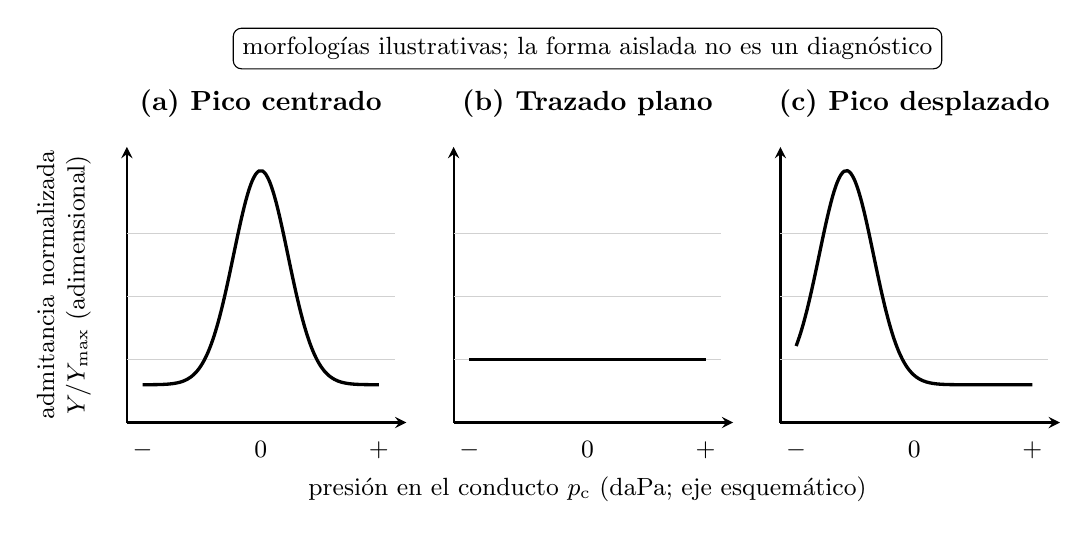
\begin{tikzpicture}[font=\small,>=stealth,x=1cm,y=1cm]
    \tikzset{
        axis/.style={->,thick},
        curve/.style={very thick},
        guide/.style={black!18,very thin}
    }

    \foreach \xshift/\title in {
        0/{(a) Pico centrado},
        4.15/{(b) Trazado plano},
        8.30/{(c) Pico desplazado}}{
        \begin{scope}[xshift=\xshift cm]
            \node[font=\bfseries] at (2.05,4.85) {\title};
            \draw[axis] (0.35,0.80) -- (3.90,0.80);
            \draw[axis] (0.35,0.80) -- (0.35,4.30);
            \draw[guide] (0.35,1.60) -- (3.75,1.60);
            \draw[guide] (0.35,2.40) -- (3.75,2.40);
            \draw[guide] (0.35,3.20) -- (3.75,3.20);
            \node[anchor=north] at (0.55,0.68) {\(-\)};
            \node[anchor=north] at (2.05,0.68) {\(0\)};
            \node[anchor=north] at (3.55,0.68) {\(+\)};
        \end{scope}
    }

    % x del gráfico = 2.05 + 0.75*u, con u en [-2,2].
    % y del gráfico = 0.80 + 3.20*Y_N.
    \draw[curve,domain=-2:2,samples=70,smooth,variable=\u]
        plot ({2.05+0.75*\u},{0.80+3.20*(0.15+0.85*exp(-(\u/0.65)^2))});
    \draw[curve] (4.70,1.60) -- (7.70,1.60);
    \draw[curve,domain=-2:2,samples=70,smooth,variable=\u]
        plot ({10.35+0.75*\u},{0.80+3.20*(0.15+0.85*exp(-((\u+1.15)/0.65)^2))});

    \node[rotate=90,align=center] at (-0.45,2.55)
        {admitancia normalizada\\\(Y/Y_{\max}\) (adimensional)};
    \node[align=center] at (6.20,-0.05)
        {presión en el conducto \(p_\mathrm{c}\)
         (\(\mathrm{daPa}\); eje esquemático)};
    \node[draw,rounded corners=3pt,fill=white,align=center]
        at (6.20,5.55)
        {morfologías ilustrativas; la forma aislada no es un diagnóstico};
\end{tikzpicture}
